\documentclass[a4paper,8pt]{extarticle} % 使用更小的字号
\usepackage[top=0.4cm,bottom=0.4cm,left=0.4cm,right=0.4cm]{geometry} % 设置页边距
\usepackage{multicol} % 多栏排版
\usepackage{amsmath}
\usepackage{amssymb}
\usepackage{physics}
\usepackage{xcolor}
\usepackage[UTF8]{ctex} % Required for inserting images
\usepackage{longtable}
\usepackage{array}
\usepackage{tabularx}
\usepackage{graphicx}
\usepackage{float}
\usepackage{listings}
\usepackage[hidelinks]{hyperref}
\usepackage{titlesec}
\usepackage{tocloft}
\usepackage{parskip} % 用于段落格式控制

% 取消首行缩进
\setlength{\parindent}{0pt}
% 设置行距
\linespread{0.9}
% 设置公式间距
\setlength{\abovedisplayskip}{2pt}
\setlength{\belowdisplayskip}{2pt}
\setlength{\abovedisplayshortskip}{2pt}
\setlength{\belowdisplayshortskip}{2pt}

% 设置段落间距
\setlength{\parskip}{0.4ex}

% 定义蓝色、红色文本、背景色
\newcommand{\bluetext}[1]{\textcolor{blue}{#1}}
\newcommand{\redtext}[1]{\textcolor{red}{#1}}
\newcommand{\yellowback}[1]{\colorbox{yellow}{#1}}

% 定义粗体
\newcommand{\black}[1]{\textbf{#1}}

% 优化多栏环境的分页设置
\raggedcolumns
\begin{document}
\begin{multicols}{3}

\redtext{一、量子力学绪论}\\
\bluetext{德布罗意关系}\\
E:粒子能量 p:粒子动量 $\nu$:粒子波频率 $\lambda$:粒子波波长 $\omega$:粒子波角频率 $k$:粒子波矢\\
波动性内部转换:$k=2\pi/\lambda$、$w=2\pi\nu$、$\hbar=h/2\pi$、$\lambda=h/p$
波矢与动量关系$k=p/\hbar$,
角频率与能量关系$\omega=E/\hbar$ \\
\bluetext{色散关系}
非相对论粒子的色散关系:$E = p^2/2m$、$\omega=hk^2/2m$\\
极端相对论粒子的色散关系:$E = cp$,
$p=E/c=h\nu/c=h/\lambda$\\
康普顿效应证明光的粒子性:散射光频率与散射角度有关\\
\redtext{二、波函数与薛定谔方程}\\
\bluetext{波函数}\\
平面波不能有限归一化,此时$|\psi(r, t)|^2$表示相对几率密度;$|\psi(r, t)|^2 = 1$时,表示波函数在全空间均匀分布\\
一维平面波波函数为$\psi(x, t) = Ae^{\frac{i}{\hbar}(px-E t)}$\\
\bluetext{态叠加原理}

态叠加:$\psi_1、\psi_2$为体系的可能状态,则$\psi=c_1\psi_1+c_2\psi_2$也是体系的可能状态,c为复常数
对一个量子体系,可用完备的状态集合${\{\psi_n\}}$来表示任意的状态$\psi$,即$\psi=\sum_n c_n\psi_n$\\
对于动量平面波,动量几率幅c(p,t)与波函数$\psi(r,t)$为傅里叶变换关系$c(p,t)=\int\psi(r,t)e^{-\frac{i}{\hbar}pr}dr$\\
动量本征函数为$\psi_p(r)=\frac{1}{(2\pi\hbar)^{3/2}}e^{\frac{i}{\hbar}pr}$\\
动量几率幅$c(p,t)$也可以完全描写单个粒子的波动性, $|c(p,t)|^2$表示动量几率密度\\
$\delta(x-x')=\frac{1}{2\pi}\int e^{ik(x-x')}dk$称为坐标本征态\\
$\psi(x)=\int_\infty\delta(x-x')\psi(x')dx'= $ \\ $\int\psi(x')\frac{1}{2\pi}\int e^{ik(x-x')}dkdx'$\\
$ = \int(\int\psi(x')\frac{1}{2\pi}e^{ikx'}dx')e^{ikx}dk=\int C(k)e^{ikx}dk $\\
$c(p)=C(k)\frac{1}{\sqrt{2\pi\hbar}}, k=\frac{p}{\hbar}$\\
\bluetext{薛定谔方程}

单粒子系统薛定谔方程:\\$i\hbar\frac{\partial}{\partial t}\psi = \hat{E}\psi = H\psi = -\frac{\hbar^2}{2\mu}\nabla^2\psi + U(\vec{r})\psi$ 
 
\bluetext{几率流密度}
几率密度:$w(\vec{r}, t) = |\psi(\vec{r}, t)|^2 = \psi^*(\vec{r}, t)\psi(\vec{r}, t)$ \\ 考虑几率密度的时变特性$\frac{\partial}{\partial t}w(\vec{r}, t)$
    
    $\frac{\partial}{\partial t}w(\vec{r}, t) = \psi^*\frac{\partial\psi}{\partial t} + \frac{\partial\psi^*}{\partial t}\psi$ 其中$\frac{\partial\psi}{\partial t}$和$\frac{\partial\psi^*}{\partial t}$两项均可从薛定谔方程(或其共轭式)中得到
    
    代入后结果:\\ $\frac{\partial}{\partial t}w(\vec{r}, t) = \frac{i\hbar}{2\mu}(\psi^*\nabla^2\psi - \psi\nabla^2\psi^*) = \frac{i\hbar}{2\mu}\nabla\cdot(\psi^*\nabla\psi - \psi\nabla\psi^*)$
    
    定义几率流密度$\vec{J} = \frac{i\hbar}{2\mu}(\psi\nabla\psi^* - \psi^*\nabla\psi)$ 有几率流守恒式$\frac{\partial w}{\partial t} + \nabla\cdot\vec{J} = 0$

    全空间几率守恒:$\int_V \frac{\partial w}{\partial t}d\tau = - \oint_S \vec{J}\cdot d\vec{S} = 0$\\

    令$W_v=\int_V w(\vec{r}, t)d\tau$为体系几率,有$W_v$为常数,全空间出现粒子的几率为1,对波函数归一化后,归一化随时间保持\\
\bluetext{定态薛定谔方程的分离变量解}

定态薛定谔方程:$H\psi = E\psi$ 也即能量本征方程,其中$H$为哈密顿算符,$E$为本征值

对应的$\psi(r)$为能量本征函数(态),有时也将$\psi_n(r, t) = \psi_n(r)\exp(-\frac{i}{\hbar}E_n t)$称为能量本征函数

含时的薛定谔方程:对应定态的本征函数为完备的状态集$\{\psi_n\}$\\
故有一般解为$\psi(r, t) = \sum_n c_n\psi_n(r)\exp(-\frac{i}{\hbar}E_n t)$

对于自由粒子波函数,动量本征态一定是能量本征态,而能量本征态不一定是动量本征态(有不同的方向)

\redtext{三、一维运动问题}

\bluetext{一维无限深方势阱}

一维运动方程:$\frac{d^2}{dx^2}\psi + \frac{2\mu(E-U(x))}{\hbar^2}\psi = 0$

一维无限深势阱的势能方程表达为: \\
$ U(x) = \begin{cases} 
0, |x| < a \\
+\infty, |x| > a
\end{cases} \quad \text{势阱外波函数为0} $\\
阱内:令$k = \frac{\sqrt{2\mu E}}{\hbar}$得$k = \frac{n\pi}{2a}, n=1,2,3,\dots$因此有体系分立能级:$E_n = \frac{\hbar^2\pi^2}{8\mu a^2}n^2$
由归一化给出$B = \frac{1}{\sqrt{a}}$因此完整定态解为 \\
$ \psi_n(x) = \begin{cases}
\frac{1}{\sqrt{a}}\sin[\frac{n\pi}{2a}(x + a)], |x| < a \\
0, |x| \geq a
\end{cases} $

根据特解(定态解),可以给出通解$\psi(x,t) = \sum_n c_n\psi_n(x)\exp(-\frac{i}{\hbar}E_nt)$ \hspace{2em} 

一维无限深方势阱的定态解为两个传播方向相反的平面波叠加形成的驻波

\bluetext{一维运动问题分析}

基态:体系中能量最低的状态,基态能量称为零点能\\
定态:即能量本征态,定态下一切力学量的本征值和相对分布不随时间改变\\
束缚态:无穷远处波函数为0的状态(即对应粒子被束缚在势阱中)vs 散射态\\
能级简并:对于相同的能量本征值$E_k$,其对应的本征函数$\psi_k$不唯一\\
共轭定理:定态薛定谔方程的解满足共轭对称性,因此若能级非简并必为实解\\
推论:对于确定的能量本征值,必有一组实解可做其全部定态解的基底\\
反射定理:势能函数关于原点对称时,其对应定态解也满足空间对称性\\
推论:对于确定的能量本征值,若该能级非简并则必有确定宇称\\
宇称:空间反射变换算符的本征值\\
非简并定理:\black{一维束缚态必为非简并态,能量分立,且势能空间对称时必有确定宇称}\\
\yellowback{证明:}假设简并,对于同一个E,方程有两个线性独立的解,而由$\psi\psi'-\psi'\psi=c(常数)$\\
对于束缚态无穷远处为0,c=0,$ln(\psi)=ln(\psi')+C$,两个解线性相关,矛盾

\bluetext{一维有限深方势阱}

$\psi(x)=\begin{cases}
Ce^{\beta x}, & (x < -a/2) \\
A\cos kx + B\sin kx, & (-a/2 < x < a/2) \\
De^{-\beta x}, & (a/2 < x)
\end{cases}$\\
其中$\beta = \sqrt{\frac{2m(V_0-E)}{\hbar^2}},k = \sqrt{\frac{2mE}{\hbar^2}}$\\
解得$E_n = \frac{\hbar^2\pi^2}{2ma^2}n^2$\\
$E_n = \frac{2\hbar^2}{ma^2}\xi_n^2, \quad 0 < \xi_1 < \frac{\pi}{2} < \xi_2 < \pi < \cdots$\\
偶宇称态(B=0,C=D)奇宇称态(A=0,C=-D)\\基态为偶宇称态,激发态奇偶相间,对应能级低于无限深势阱
\\束缚态的能级总数为$N=1+[\frac{a}{\hbar\pi}\sqrt{2mV_0}]$\\
\bluetext{三维无限深方势阱}
按照直角坐标系分离变量$\psi(r) = X(x)Y(y)Z(z)$\\
求解得到:$E_{n,m,l} = \frac{\hbar^2\pi^2}{2m}(n^2/a^2 + m^2/b^2 + l^2/c^2)$\\
对应的波函数为:\\$\psi_{n,m,l}(x,y,z) = \sqrt{\frac{8}{abc}}\sin(\frac{n\pi x}{a})\sin(\frac{m\pi y}{b})\sin(\frac{l\pi z}{c})$\\
二维极限:c趋近于0,l=1和l=2能级差距极大,粒子冻结在l=1能态,一维极限类似\\
\bluetext{平行平面极板}\\
粒子在x,y方向上自由,在z方向上受限,波函数为\\
$\psi(x,y,z) = C\exp(i(k_xx+k_yy))\sin(k_zz),k_z=\frac{n\pi}{a}$ kx和ky任意实数(连续)\\
能量分立的原理是束缚态条件(无穷远处波函数为0)只在分立值成立\\
\bluetext{一维线性谐振子}\\
势能方程为$U(x) = \frac{1}{2}m\omega^2x^2$\\
能级为$E_n = (n+\frac{1}{2})\hbar\omega$\\
归一化波函数为\\$\psi_n(x) = N_nH_N(\alpha x)\exp(-\alpha^2x^2/2)$\\
其中$\alpha = \sqrt{\frac{m\omega}{\hbar}},N_n = \sqrt{\frac{\alpha}{\sqrt{\pi}2^n n!}}$\\
常用谐振子状态:\\
\begin{figure}[H]
    \vspace{-0.5cm}
    \centering
    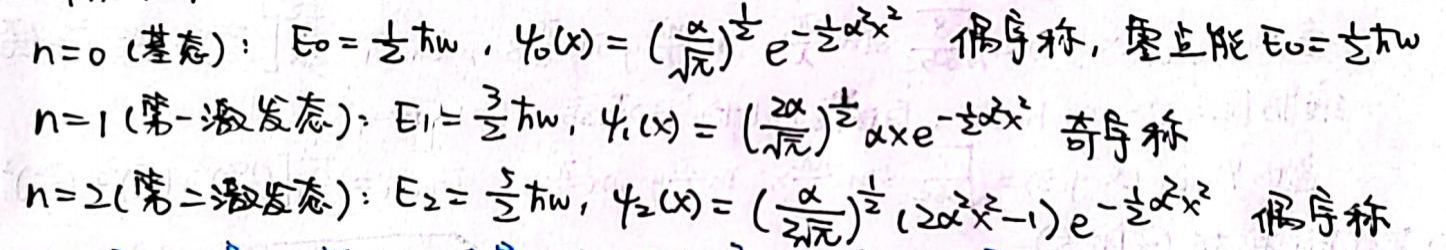
\includegraphics[width=0.32\textwidth]{images/31.png}
    \vspace{-0.6cm}
\end{figure}
谐振子定态必为束缚态\\
相干态定义:将基态波包平移(中心从x=0移到x=x0)得到的态\\
特点:1.不是能量本征态 2.不是定态,几率密度随时间变化 3. 波包形状保持不变,波包中心周期性变化\\
$|\psi(x,t)|^2=|\psi(x-x_0 cos\omega t)|^2$

\bluetext{量子隧穿效应}

背景:粒子可以进入E<U的区域,由定态薛定谔方程,这一区域的波函数可以不为0\\
一维散射问题的一般性描述:无穷远处波函数不一定为0,只考虑定态问题\\
\begin{figure}[H]
    \vspace{-0.5cm}
    \centering
    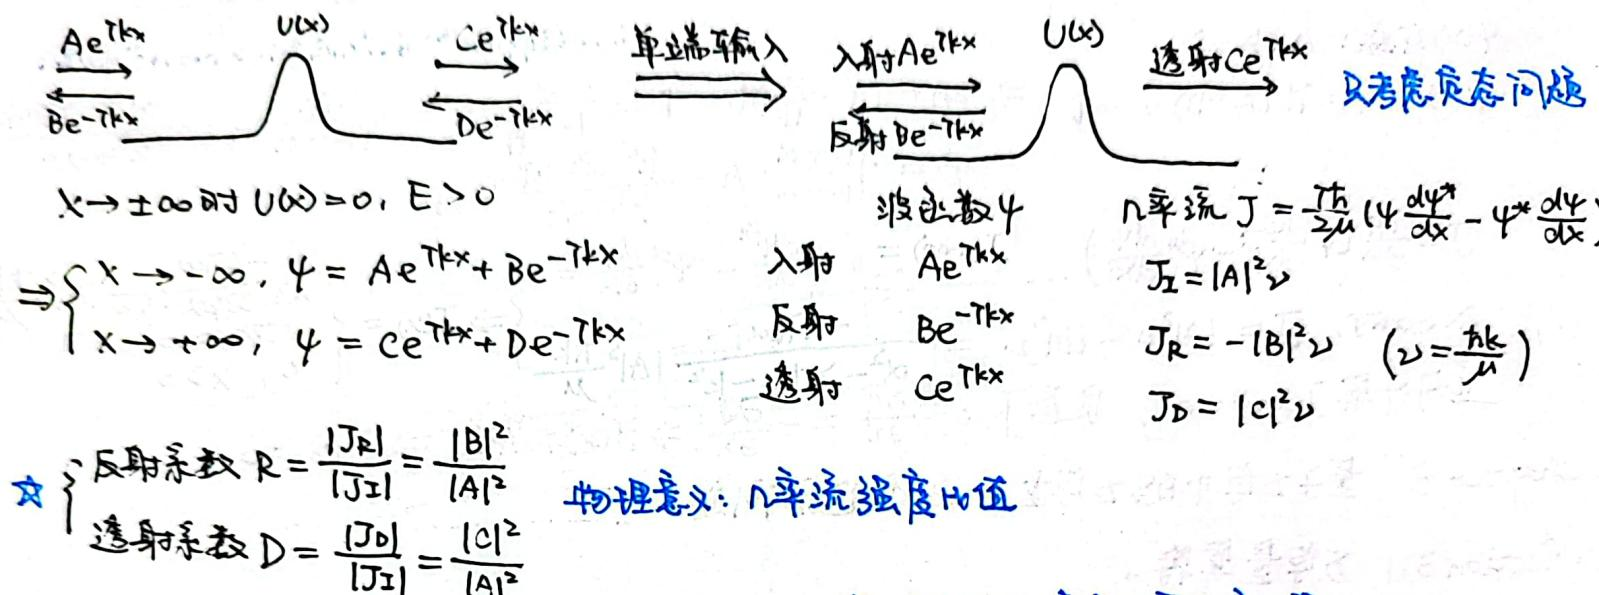
\includegraphics[width=0.32\textwidth]{images/32.png}
    \vspace{-0.6cm}
\end{figure}
定态下所有一维散射问题均有R+D=1\\
\begin{figure}[H]
    \vspace{-0.5cm}
    \centering
    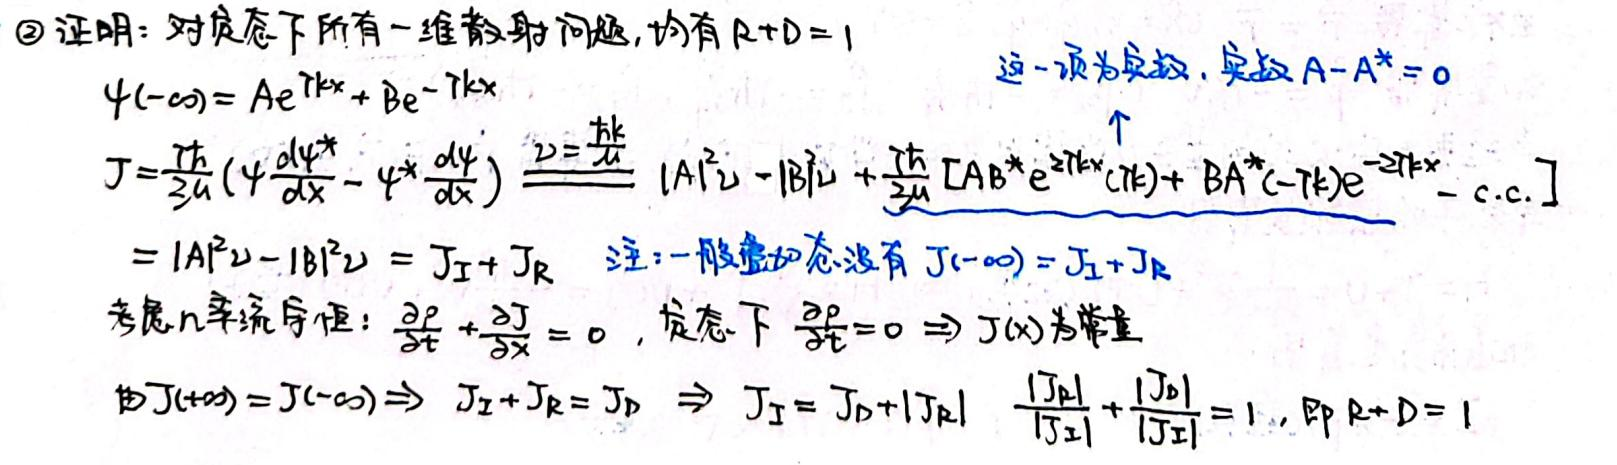
\includegraphics[width=0.32\textwidth]{images/33.png}
    \vspace{-0.6cm}
\end{figure}

\bluetext{半无限宽势垒}

$\begin{cases}
    U(x) = 0, \psi (x)=Ae^{ikx}+Be^{-ikx}, x \leq 0 \\
    U(x) = U_0, \psi (x)=De^{-\alpha x}, x > 0
    \end{cases}$\\
$k=\sqrt{\frac{2mE}{\hbar^2}},\alpha=\sqrt{\frac{2m(U_0-E)}{\hbar^2}}$\\

\bluetext{方势垒穿透}

$\frac{B}{A}=\frac{(k^2+\alpha^2)sh(\alpha a)}{(k^2-\alpha^2)sh(\alpha a)+2ik\alpha ch(\alpha a)}$\\
$\frac{C}{A}=\frac{2ik\alpha e^{-ika}}{(k^2-\alpha^2)sh(\alpha a)+2ik\alpha ch(\alpha a)}$\\
重要结论1:根据几率流守恒定律,得到定态下J(x)为常量\\
重要结论2:透射系数$D \approx D_0\exp(-2\alpha a)$,其中$\alpha = \sqrt{\frac{2m(U_0-E)}{\hbar^2}}$\\
\redtext{四、力学量算符与氢原子}\\
\bluetext{力学量算符}\\
算符:作用于波函数,将其变为另一个函数的运算\\
哈密顿量算符:$H = -\frac{\hbar^2}{2m}\nabla^2 + U(\vec{r})$\\
角动量算符:$\vec{L} = \vec{r}\times\vec{p} = -i\hbar\vec{r}\times\nabla$\\
算符$\hat{F}$的本征方程为$\hat{F}(\vec{r}, -i\hbar\nabla)\psi_\lambda(\vec{r}) = \lambda\psi_\lambda(\vec{r})$\\
测量假设(量子力学基本假设1):本征值的集合对应力学量实际可能的测量值集合\\
厄密性质:$\int\Psi^*(\hat{F}\psi) d\tau = \int(\hat{F}\Psi)^*\psi d\tau$\\
($d\tau$为体积元,对于三维空间即为$dxdydz$)\\
即 $F^+ = F$, 则算符为厄米算符\\
用内积表示为 $(u,Fv) = (Fu,v)$\\
其中厄米共轭的定义: $(u,F^{+}v) \equiv (Fu,v)$ \\
积分表示为 $\int\Psi^*(\hat{F}\psi) d\tau = \int(\hat{F}^{+}\Psi)^*\psi d\tau$\\
性质1:$(\hat{A}\hat{B})^{+}= \hat{B}^{+}\hat{A}^{+}$\\
性质2:$(\hat{A}^{+})^{+} = \hat{A}$\\
性质3:若$\hat{F}=C$为复常数,则$\hat{F}^{+}=C^{*}$\\
重要结论:厄米算符的本征值均为实数,力学量算符均为厄米算符\\
\yellowback{证明:}\\
$\int \psi^*(F\phi)\cdot d\tau = \int (F\psi)^*\phi\cdot d\tau, \text{ 取 }\phi=\psi$\\
这样得到:\\
$\int \psi^*(F\psi)\cdot d\tau = \int (F\psi)^*\psi\cdot d\tau$\\
$\hat{F}\psi = \lambda\psi$\\
$\text{左边} = \lambda\int \psi^*\psi\cdot d\tau$
$\text{右边} = \lambda^*\int \psi^*\psi\cdot d\tau$
$\lambda = \lambda^* \text{ (是实数)}$\\
\bluetext{动量算符}
本征方程为$\hat{p}\psi = p\psi=-i\hbar\nabla\psi$\\
其解为$\psi_p(\vec{r}) = Ce^{i\vec{p}\cdot\vec{r}/\hbar}$\\
1.函数规格化--归一不同动量本征函数的内积到δ函数:\\
$\int\psi^*_{p'}(\vec{r})\psi_{p}(\vec{r})d\tau = \delta^3(\vec{p}-\vec{p'})$\\
此外:$\int\psi^*_{p}(\vec{r'})\psi_{p}(\vec{r})d\tau = \delta^3(\vec{r'}-\vec{r})$\\
关键积分:$\int e^{i\vec{p}\cdot\vec{r}/\hbar}d\tau = (2\pi\hbar)^3\delta^3(\vec{p})$\\
得到归一化系数$C = \frac{1}{(2\pi\hbar)^{3/2}}$\\
2.箱归一化--将连续谱动量转化为离散谱动量(人为添加边界条件)\\
此时限制相对箱壁上对应点有相同值,可以归一化内积到1\\
$\psi_{\vec{p}}=\frac{1}{L^{3/2}}exp(i\vec{p}\cdot\vec{r}/\hbar)$\\
取点A(-L/2,0,0),B(L/2,0,0),$\psi_A=\psi_B$\\
=> $Cexp(-ip_xL/2\hbar)=Cexp(ip_xL/2\hbar)$\\
=> $exp(ip_xL/\hbar)=1$,即$p_x=\frac{2\pi\hbar n_x}{L}$\\
自由粒子波函数为$\psi_p(\vec{r},t)=Ae^{i(\vec{p}\cdot\vec{r}-Et)/\hbar}=\psi_p(\vec{r})e^{-iEt/\hbar}$\\
\yellowback{证明:}动量算符满足厄密性\\
$\int \psi^*(\hat{p}\phi)\cdot dx = \int(\hat{p}\psi)^*\phi\cdot dx$\\
$\int \psi^*(-i\hbar\frac{d}{dx})\phi\cdot dx = \int(-i\hbar\frac{d}{dx}\psi)^*\phi\cdot dx$\\
$\Rightarrow \int dx(\psi^*\frac{d}{dx}\phi + \frac{d}{dx}\psi^*\phi) = \int dx\frac{d}{dx}(\psi^*\phi)$\\
(1) 若假设无穷远处波函数为零,则厄密性满足。\\
(2) 若满足箱归一化条件,即:\\
$\psi^*(L/2)\phi(L/2) = \psi^*(-L/2)\phi(-L/2) \quad (L \rightarrow +\infty)$
则厄密性也满足。

\bluetext{角动量算符}

$\vec{L} = \begin{vmatrix} \hat{i} & \hat{j} & \hat{k} \\ x & y & z \\ -i\hbar\partial_x & -i\hbar\partial_y & -i\hbar\partial_z \end{vmatrix}$\\
引入球坐标转换:\\$x = r\sin\theta\cos\phi, y = r\sin\theta\sin\phi, z = r\cos\theta$\\
$\vec{L} = \vec{r} \times \vec{p} = -i\hbar\vec{r} \times \nabla = -i\hbar\vec{e}_r \times \nabla$
$= -i\hbar\vec{e}_r \times (\vec{e}_r \frac{\partial}{\partial r} + \vec{e}_\theta \frac{1}{r}\frac{\partial}{\partial \theta} + \vec{e}_\varphi \frac{1}{r\sin\theta}\frac{\partial}{\partial \varphi})$
利用单位矢量的叉乘关系:
$\vec{e}_r \times \vec{e}_r = 0, \quad \vec{e}_r \times \vec{e}_\theta = \vec{e}_\varphi, \quad \vec{e}_r \times \vec{e}_\varphi = -\vec{e}_\theta$
得到:
$\vec{L} = -i\hbar(\vec{e}_\varphi \frac{\partial}{\partial \theta} - \vec{e}_\theta \frac{1}{\sin\theta}\frac{\partial}{\partial \varphi})$
\begin{figure}[H]
    \centering
    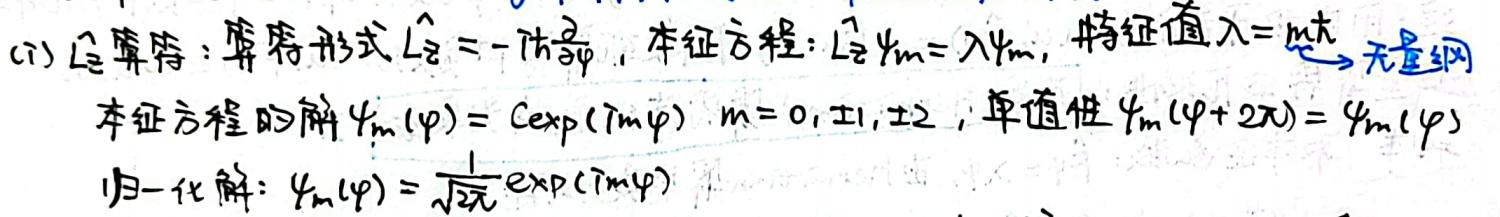
\includegraphics[width=0.32\textwidth]{images/6.png}
    \vspace{-0.6cm}
\end{figure}
\begin{figure}[H]
    \centering
    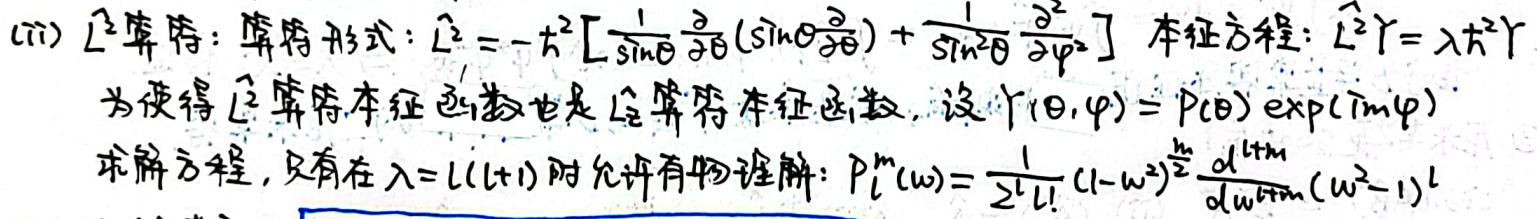
\includegraphics[width=0.32\textwidth]{images/7.png}
    \vspace{-0.6cm}
\end{figure}
重要结论:球谐函数$Y_{l,m}(\theta,\phi)$是角动量算符$L^2,L_z$的共同本征函数\\
不考虑自旋时,$L^2$的简并度为2l+1\\
球谐函数正交归一;\\
共轭性质:$Y_{l,m}^*(\theta,\phi) = (-1)^mY_{l,-m}(\theta,\phi)$\\
\begin{figure}[H]
    \vspace{-0.5cm}
    \centering
    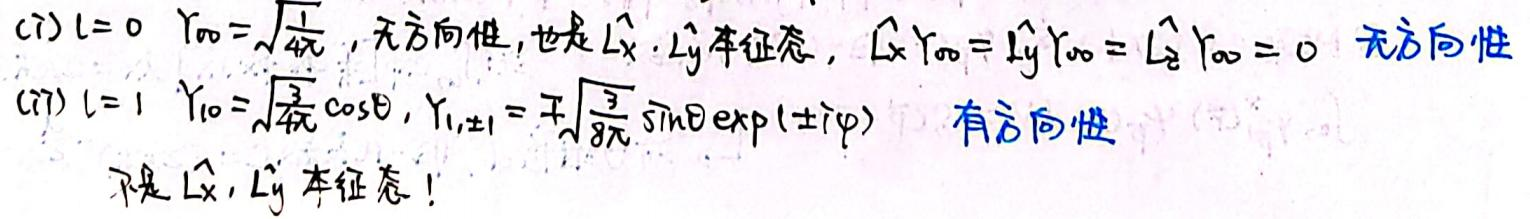
\includegraphics[width=0.32\textwidth]{images/8.png}
    \vspace{-0.6cm}
\end{figure}
$L_z=xp_y-yp_x,L_x=yp_z-zp_y,L_y=zp_x-xp_z$\\
\bluetext{氢原子模型}

中心力场模型:运动分解为质心运动+相对质心运动,通过分离变量,只关心相对运动\\
\begin{figure}[H]
    \vspace{-0.5cm}
    \centering
    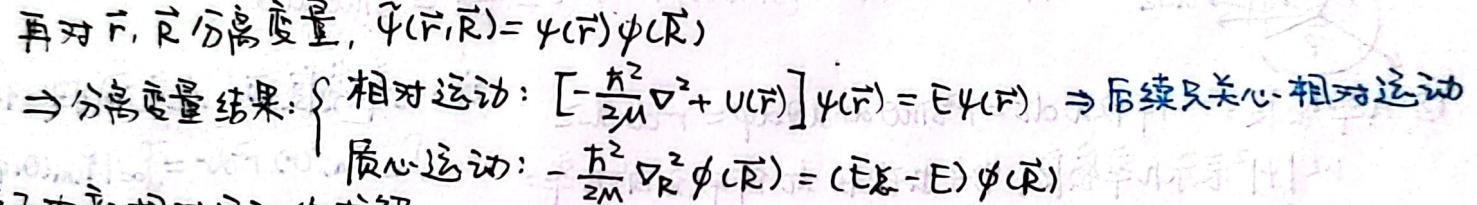
\includegraphics[width=0.32\textwidth]{images/30.png}
    \vspace{-0.6cm}
\end{figure}
之后分离变量$\psi(r,\theta,\phi) = R(r)Y(\theta,\phi)$\\
根据哈密顿量表达式将动量分为径向动量和转动动量\\
$\begin{cases}
    \frac{\hat{L}^2Y(\theta,\phi)}{Y(\theta,\phi)} = \lambda\hbar^2\left[\text{以前级数求解得}\lambda = l(l+1)\right] \\[2ex]
    -\frac{\hbar^2}{2\mu r^2}\frac{d}{dr}\left(r^2\frac{dR}{dr}\right) + \left[U(r) + \frac{\lambda\hbar^2}{2\mu r^2}\right]R = ER(r)
    \end{cases}$\\
得到能量本征值,有束缚态解,离散谱(E>0时非束缚态,连续谱)\\
$E = -\frac{m_e}{2\hbar^2n^2}(\frac{Ze^2}{4\pi\epsilon_0})^2$,$n=1,2,3,\dots$,氢原子Z=1\\
其中$n=n_r+l+1$,$l=0,1,2,\dots$,$n_r$为径量子数\\
氢原子能谱:$E_n = -\frac{13.6}{n^2}eV$\\
宇称性质只与角量子数l有关,l为奇数时为奇宇称,l为偶数时为偶宇称\\
$\psi_{n,l,m}(-\vec{r}) = (-1)^l\psi_{n,l,m}(\vec{r})$\\
$\psi_{nlm}(r,\theta,\phi) = \sqrt{\left(\frac{2}{na}\right)^3 \frac{(n-l-1)!}{2n(n+l)!}} \times \left(\frac{2r}{na}\right)^l e^{-\frac{r}{na}} L_{n-l-1}^{2l+1}\left(\frac{2r}{na}\right)Y_{lm}(\theta,\phi)$\\
$\psi_{100} = \sqrt{\frac{1}{\pi a^3}}\exp\left(-\frac{r}{a}\right) = \sqrt{\frac{4}{a^3}}\exp\left(-\frac{r}{a}\right)Y_{00}(\theta,\phi)$\\
$\psi_{200} = \sqrt{\frac{1}{2a^3}}\left(1-\frac{r}{2a}\right)\exp\left(-\frac{r}{2a}\right)Y_{00}(\theta,\phi)$\\
$\psi_{21m} = \sqrt{\frac{1}{6a^3}}\left(\frac{r}{2a}\right)\exp\left(-\frac{r}{2a}\right)Y_{1m}(\theta,\phi),(m=1,0,-1)$\\
\redtext{五、本征函数系与测量问题}

\bluetext{本征函数系}

正交性定理:同一个厄米算符属于不同本征值的本征函数彼此正交\\
共同本征函数定理:若两个算符F,G满足$[F,G]=0$,则F,G有组成完全系的共同本征函数\\
\yellowback{证明}:
\begin{figure}[H]
    \vspace{-0.5cm}
    \centering
    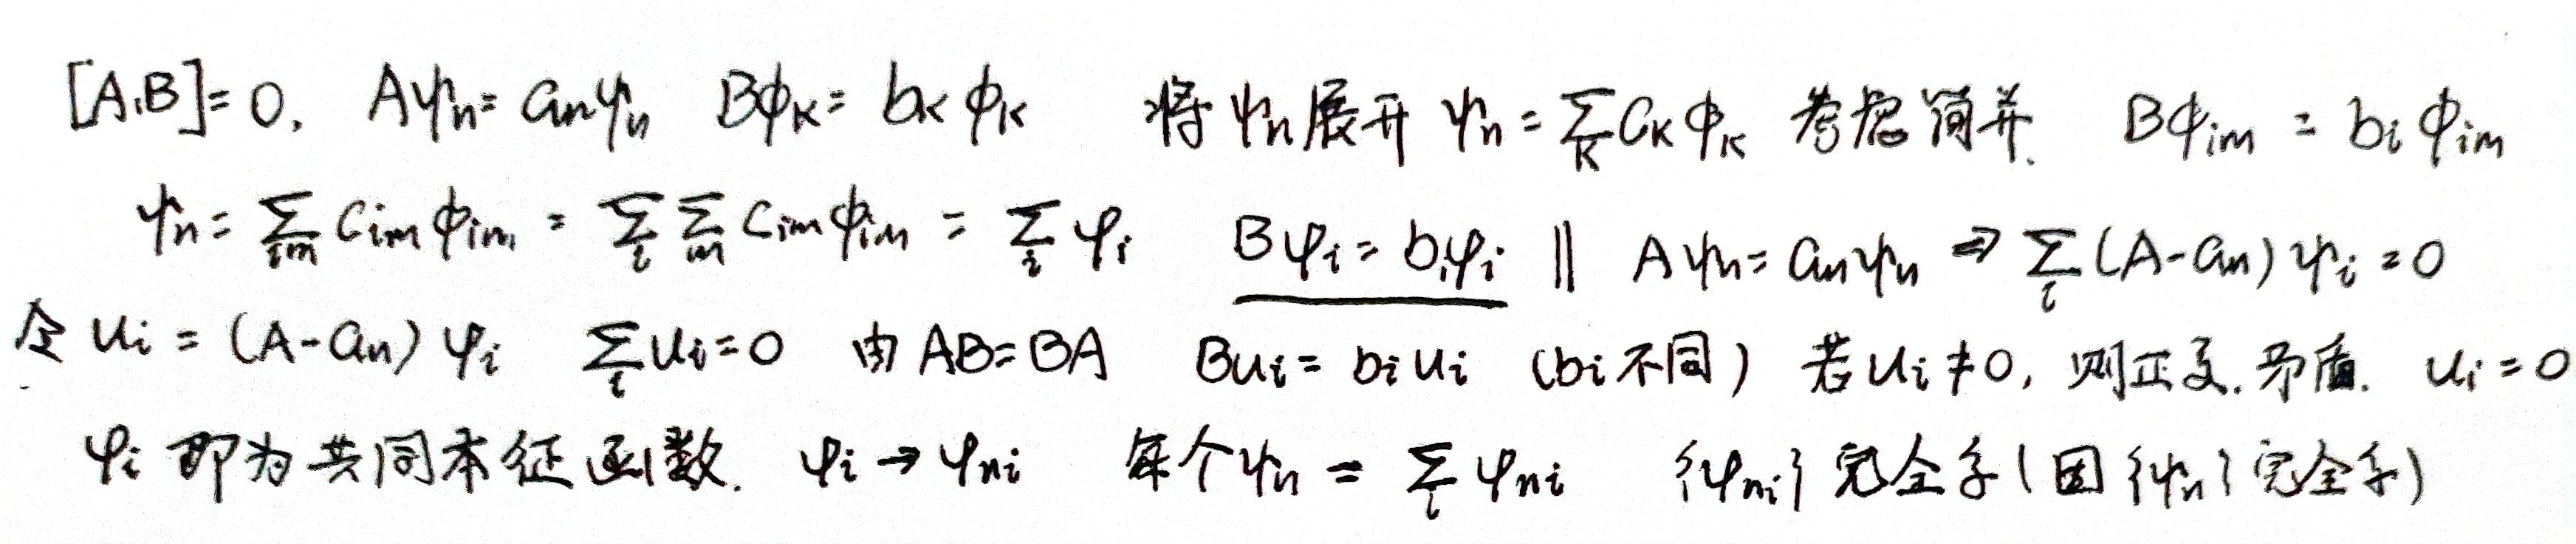
\includegraphics[width=0.32\textwidth]{images/34.jpg}
    \vspace{-0.6cm}
\end{figure}
力学量完全集(完备算符集):相互之间两两对易,能够对一个量子体系全部状态进行非简并
分类标记的最少数目的力学量算符\\
力学量完全集的共同本征函数系必然为正交函数系
对易相关: $[x,p] = i\hbar, [L_x,L_y] = i\hbar L_z$,
$[A,BC]=B[A,C]+[A,B]C$\\
三维空间单粒子选取方法:坐标$\{x,y,z\}$动量$\{px,py,pz\}$转动$\{Lz,L^2\}$
原子状态:$H,L^2,L_z,S_z$\\
\bluetext{算符与力学量的关系}

力学量平均值计算:\\ $\bar{F} = \sum_n \lambda_n W(\lambda_n) = \sum_n \lambda_n |C_n|^2, \quad C_n = \int \phi_n^*(x) \psi(x,t) dx$\\
平均值公式:$\bar{F(t)} = \int \psi^*(x,t) \hat{F} \psi(x,t) dx$\\
若未归一化,可用$\frac{\int \psi^*(x,t) \hat{F} \psi(x,t) dx}{\int \psi^*(x,t) \psi(x,t) dx}$\\
\yellowback{证明}:将波函数用对应力学量F的本征函数系展开
\begin{figure}[H]
    \vspace{-0.5cm}
    \centering
    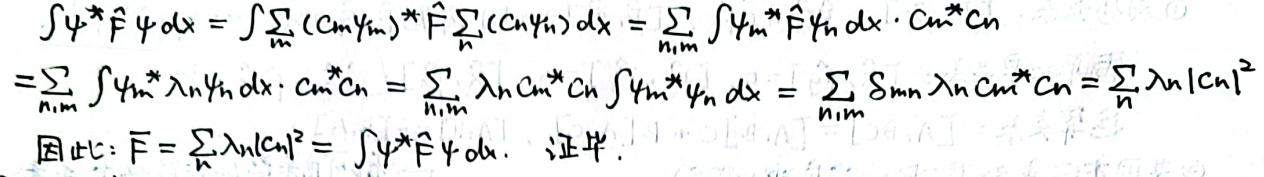
\includegraphics[width=0.32\textwidth]{images/9.png}
    \vspace{-0.6cm}
\end{figure}
测量问题总结:测量值为本征值,测量几率由几率幅(波函数)决定

\bluetext{不确定关系}
厄密算符$\Delta F = \hat{F}-\bar{F}$
有$\bar{(\Delta F)^2} = \bar{\hat{F}^2} - \bar{F}^2$(不确定度)\\
不确定关系:若不对易算符$[\hat{F},\hat{G}] = \hat{F}\hat{G}-\hat{G}\hat{F} = i\hat{C}$\\
则有$\bar{(\Delta F)^2}\bar{(\Delta G)^2} \geq \frac{1}{4}|\bar{\hat{C}}|^2$\\
\yellowback{证明}:利用积分非负性:
\begin{figure}[H]
    \vspace{-0.5cm}
    \centering
    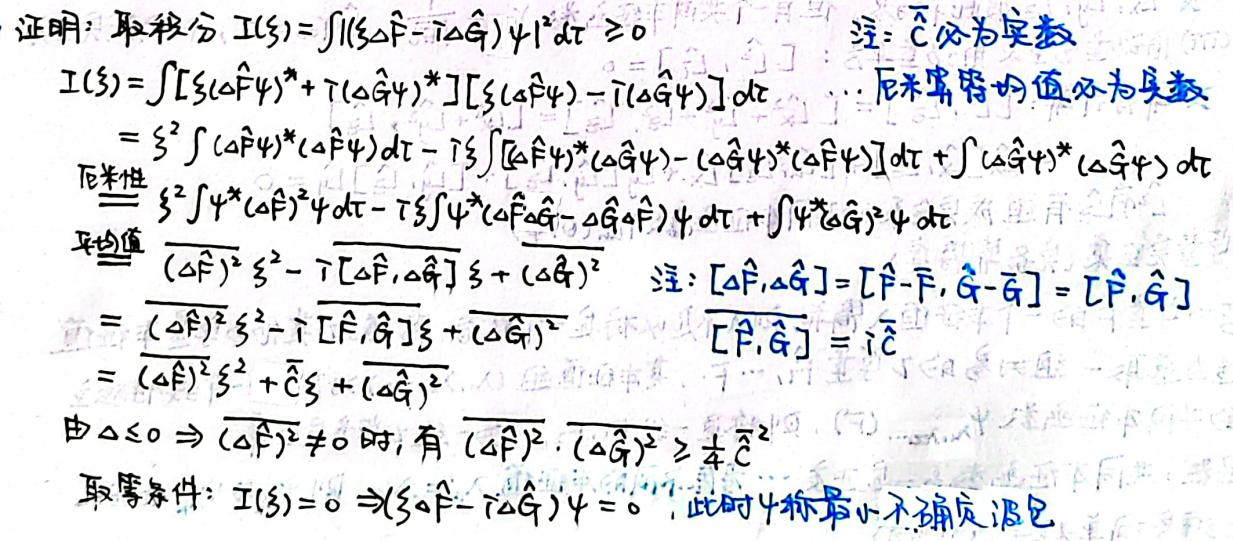
\includegraphics[width=0.32\textwidth]{images/28.png}
    \vspace{-0.6cm}
\end{figure}
线性谐振子零点能\yellowback{证明}:
\begin{figure}[H]
    \vspace{-0.5cm}
    \centering
    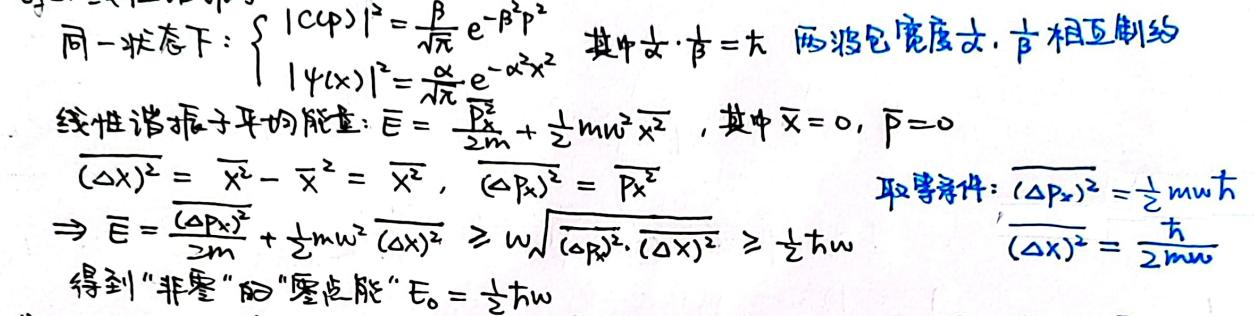
\includegraphics[width=0.32\textwidth]{images/3.png}
    \vspace{-0.6cm}
\end{figure}
\bluetext{守恒量}

力学量期望随时间的变化:考虑力学量期望值对时间的导数:\\
\begin{figure}[H]
    \vspace{-0.5cm}
    \centering
    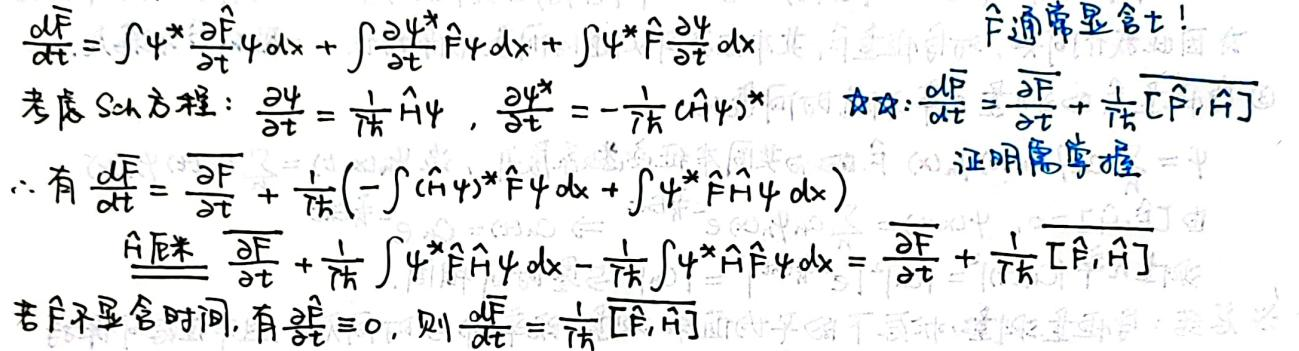
\includegraphics[width=0.32\textwidth]{images/29.png}
    \vspace{-0.6cm}
\end{figure}
守恒量:若F不显含时间且与H对易,则力学量期望值不随时间改变,称F为守恒量\\
守恒量的例子:自由粒子中p、H;一维无限深势阱中p、H;一维谐振子只有H;氢原子中$L^2$、Lz、H\\
\bluetext{测量与运动}

重要结论1:定态下,不显含时的任意力学量平均值与测量几率不随时间变化\\
重要结论2:守恒量F的本征态可以随时间保持\\
重要结论3:守恒量F的测量几率和分布不随时间改变\\
总结:守恒量都不变,定态下不显含时力学量不变\\
\redtext{六、量子力学中的矩阵表象}

\bluetext{态和力学量的表象}

表象:量子力学中态和力学量的具体表示方式(可理解为波函数的自变量)\\
此前我们使用的$\psi(\vec{r},t)$对应坐标表象,同一种态在不同表象中波函数不同,但意义相同
力学量在不同表象中表现为作用于对应波函数的算符

\bluetext{量子力学的矩阵形式}

算符的矩阵形式:$F_{mn}= \int u_m^*(x) \hat{F}u_n(x) dx$\\
力学量算符在自身表象中为对角阵\\
\begin{figure}[H]
    \vspace{-0.5cm}
    \centering
    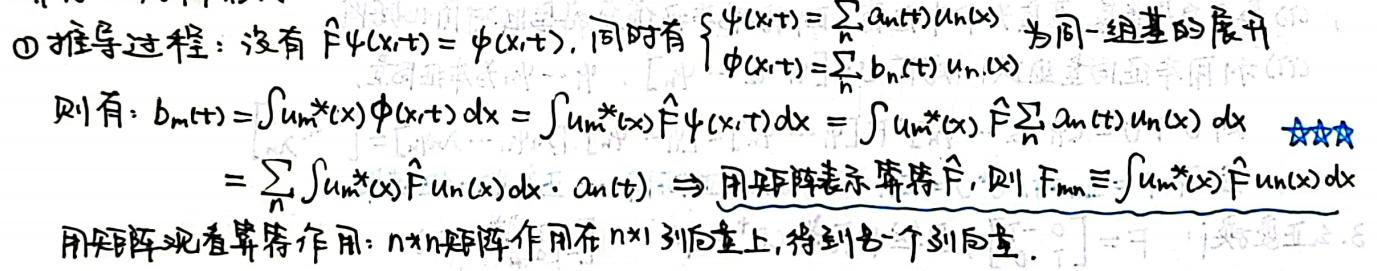
\includegraphics[width=0.32\textwidth]{images/13.png}
    \vspace{-0.6cm}
\end{figure}
\begin{figure}[H]
    \vspace{-0.5cm}
    \centering
    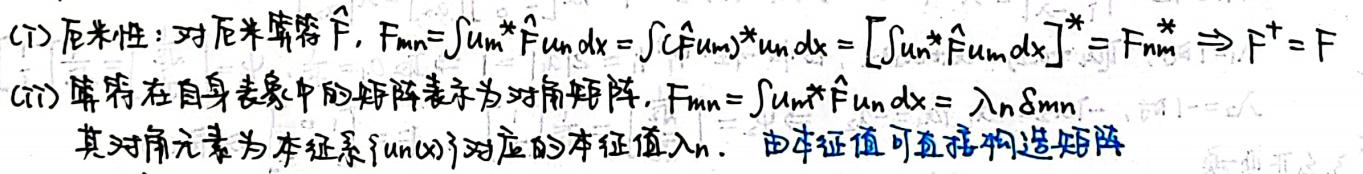
\includegraphics[width=0.32\textwidth]{images/14.png}
    \vspace{-0.6cm}
\end{figure}
用矩阵形式表达量子力学的重要公式:期望值公式、本征值方程、薛定谔方程\\
\begin{figure}[H]
    \vspace{-0.5cm}
    \centering
    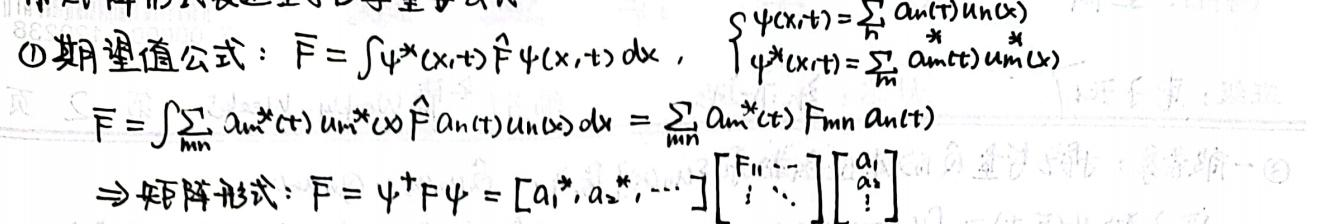
\includegraphics[width=0.35\textwidth]{images/15.png}
    \vspace{-0.6cm}
\end{figure}
\begin{figure}[H]
    \vspace{-0.5cm}
    \centering
    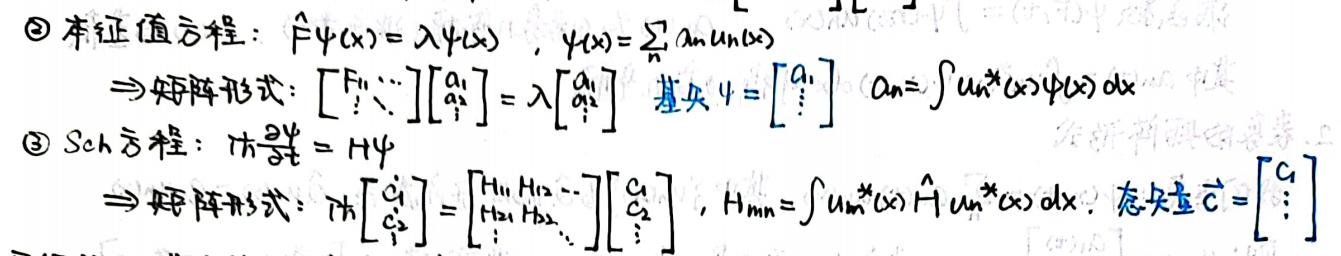
\includegraphics[width=0.32\textwidth]{images/16.png}
    \vspace{-0.6cm}
\end{figure}
用矩阵形式求解力学量的本征值--久期方程和对角化F矩阵
\begin{figure}[H]
    \vspace{-0.6cm}
    \centering
    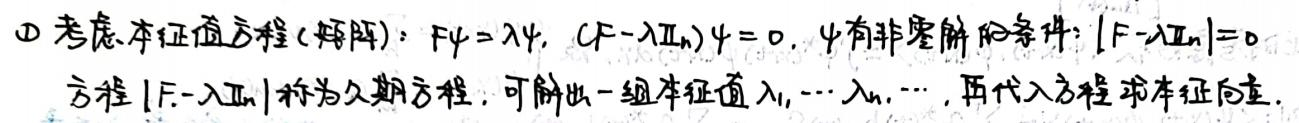
\includegraphics[width=0.32\textwidth]{images/17.png}
    \vspace{-0.6cm}
\end{figure}
\begin{figure}[H]
    \centering
    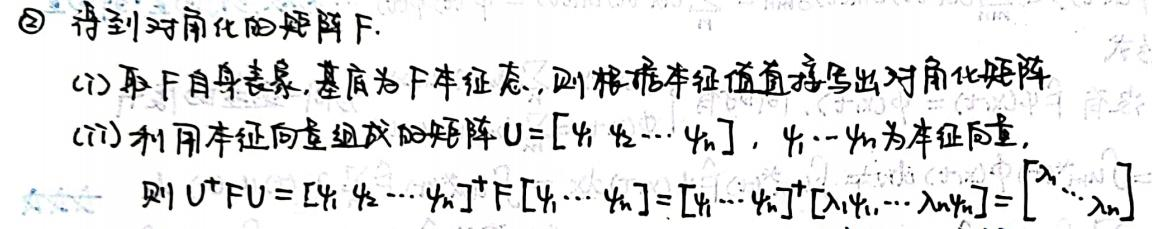
\includegraphics[width=0.32\textwidth]{images/18.png}
    \vspace{-0.6cm}
\end{figure}
表象变换:不同表象之间变换的转移矩阵S\\
矩阵表象主要作用:便于表象变换和求解测量问题

\bluetext{Dirac符号系统}

Dirac符号是不考虑表象情况下,对量子力学的重新书写\\
\begin{figure}[H]
    \vspace{-0.5cm}
    \centering
    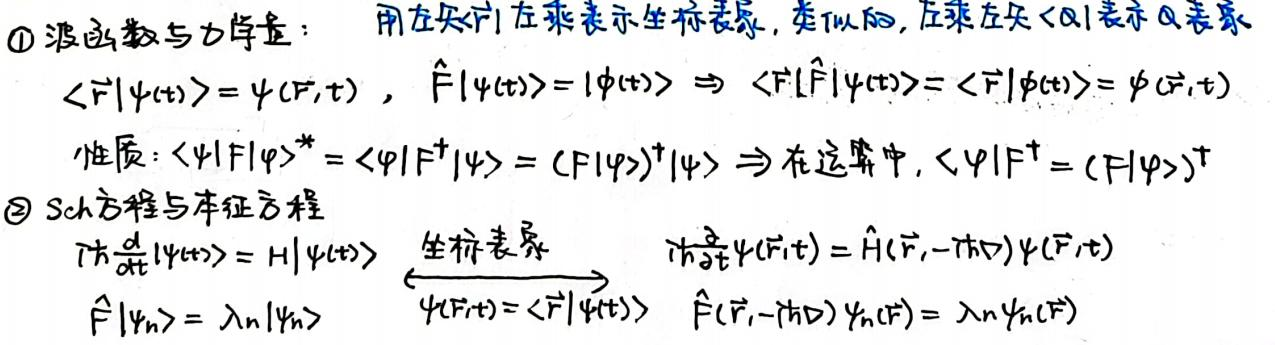
\includegraphics[width=0.32\textwidth]{images/19.png}
    \vspace{-0.6cm}
\end{figure}
\begin{figure}[H]
    \vspace{-0.5cm}
    \centering
    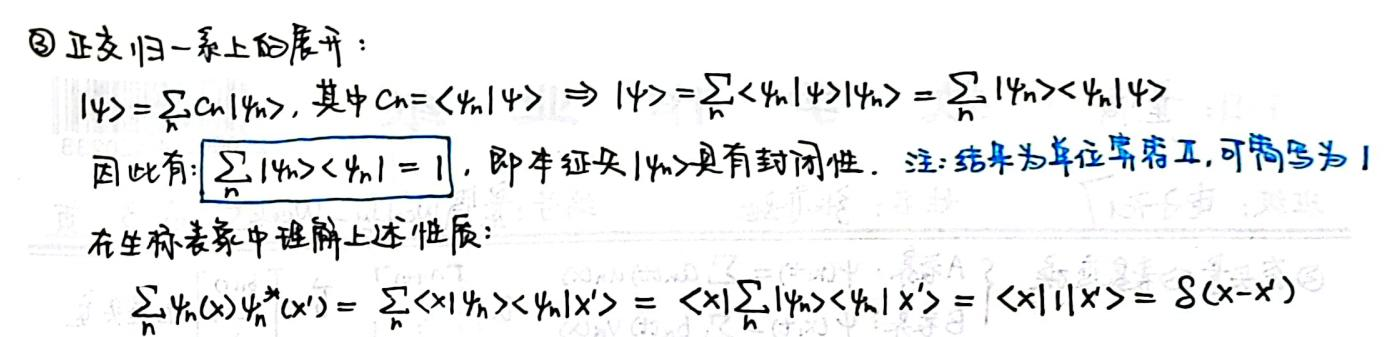
\includegraphics[width=0.32\textwidth]{images/20.png}
    \vspace{-0.6cm}
\end{figure}
\begin{figure}[H]
    \vspace{-0.5cm}
    \centering
    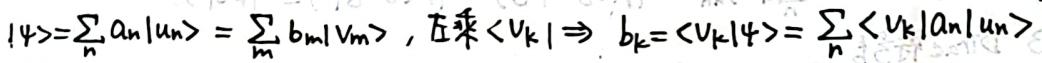
\includegraphics[width=0.32\textwidth]{images/21.png}
    \vspace{-0.6cm}
\end{figure}
\bluetext{谐振子升降算符}

对于一维线性谐振子难以求解的问题,我们给出\black{占有数表象下利用升降算符}简便求解的方法\\
对谐振子的哈密顿量做无量纲化:
\begin{figure}[H]
    \vspace{-0.5cm}
    \centering
    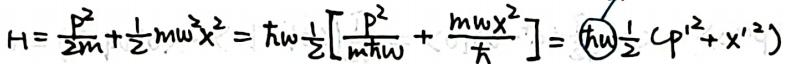
\includegraphics[width=0.32\textwidth]{images/22.png}
    \vspace{-0.6cm}
\end{figure}
\begin{figure}[H]
    \vspace{-0.5cm}
    \centering
    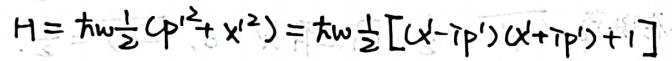
\includegraphics[width=0.32\textwidth]{images/23.png}
    \vspace{-0.6cm}
\end{figure}
\begin{figure}[H]
    \vspace{-0.5cm}
    \centering
    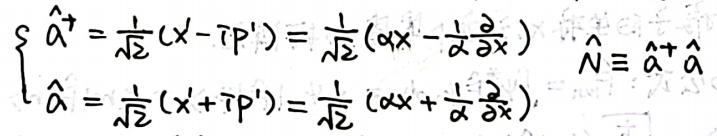
\includegraphics[width=0.32\textwidth]{images/24.png}
    \vspace{-0.6cm}
\end{figure}
$\hat{a}^\dagger$为$\hat{a}$的共轭算符,满足关系$[\hat{a},\hat{a}^\dagger]=1$\\
$\hat{N} = \hat{a}^{\dagger}\hat{a}, \text{ 设 }|\psi_n\rangle \text{ 为 } \hat{N} \text{ 的本征矢,} \text{ 简记作 } |n\rangle,$\\
$ \text{ 有 } \hat{N}|n\rangle = n|n\rangle$\\
$ n \text{ 称为占有数,} \hat{N} \text{ 表象称为占有数表象,} $\\
$\text{ 显然 } \hat{H}|n\rangle = \hbar\omega(\hat{N}+\frac{1}{2})|n\rangle = \hbar\omega(n+\frac{1}{2})|n\rangle$\\
\black{说明$|n\rangle$也是能量本征态}\\
\begin{figure}[H]
    \vspace{-0.5cm}
    \centering
    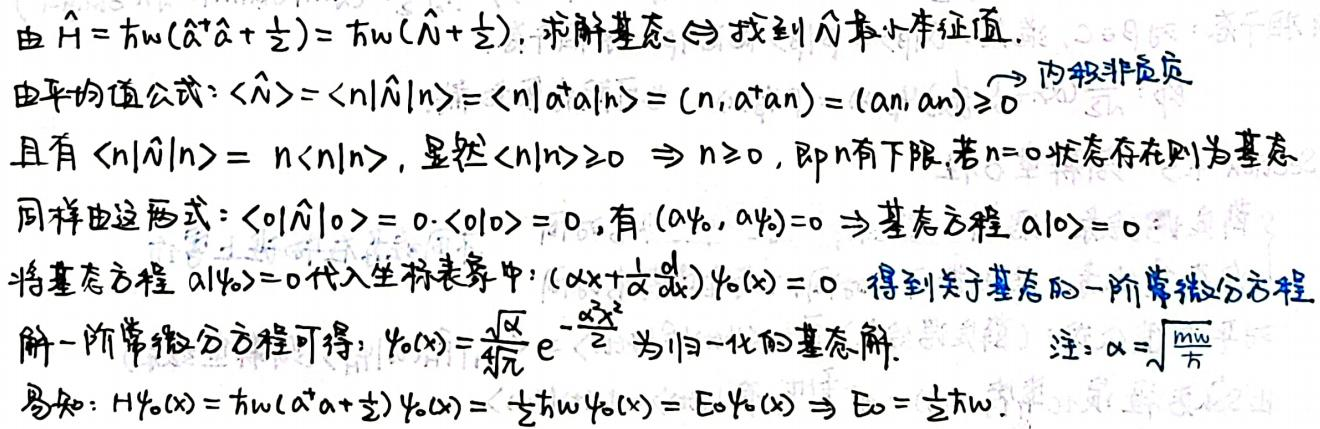
\includegraphics[width=0.32\textwidth]{images/25.png}
    \vspace{-0.6cm}
\end{figure}
升降性质:$\hat{a}|n\rangle = \sqrt{n}|n-1\rangle, $\\
$ \hat{a}^\dagger|n\rangle = \sqrt{n+1}|n+1\rangle$\\
\begin{figure}[H]
    \vspace{-0.5cm}
    \centering
    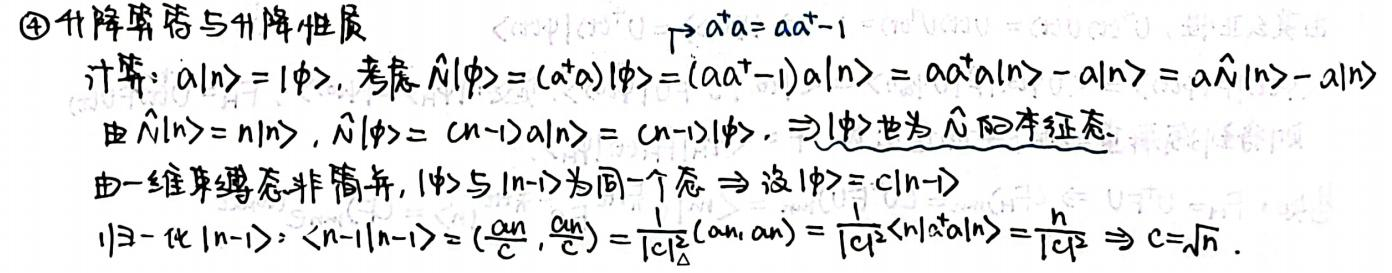
\includegraphics[width=0.32\textwidth]{images/26.png}
    \vspace{-0.6cm}
\end{figure}
推导其他本征态:\\
\begin{figure}[H]
    \vspace{-0.5cm}
    \centering
    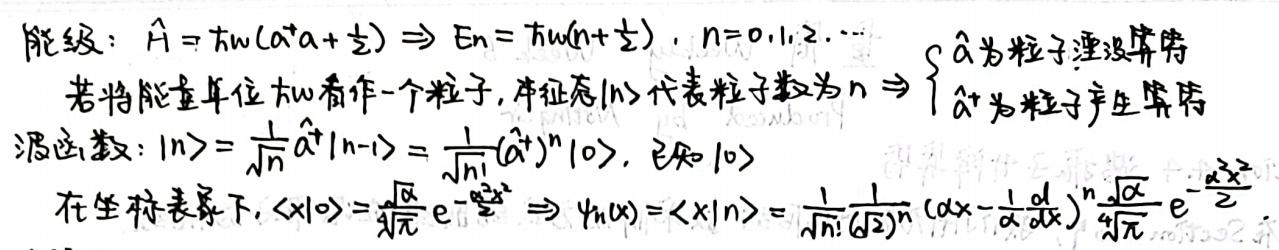
\includegraphics[width=0.32\textwidth]{images/27.png}
    \vspace{-0.6cm}
\end{figure}
\redtext{七、电子的自旋与角动量}

\bluetext{电子自旋}

电子有轨道磁矩$\mu_L = -\frac{e}{2m_e}L$,自旋磁矩$\mu_S = -\frac{e}{m_e}S$\\
核心:自旋类似角动量,但是纯内在构造算符,没有经典对应\\
引入自旋后,氢原子的波函数需要考虑的量子数增加到4个\\
自旋算符与旋量波函数:\\
\begin{figure}[H]
    \vspace{-0.5cm}
    \centering
    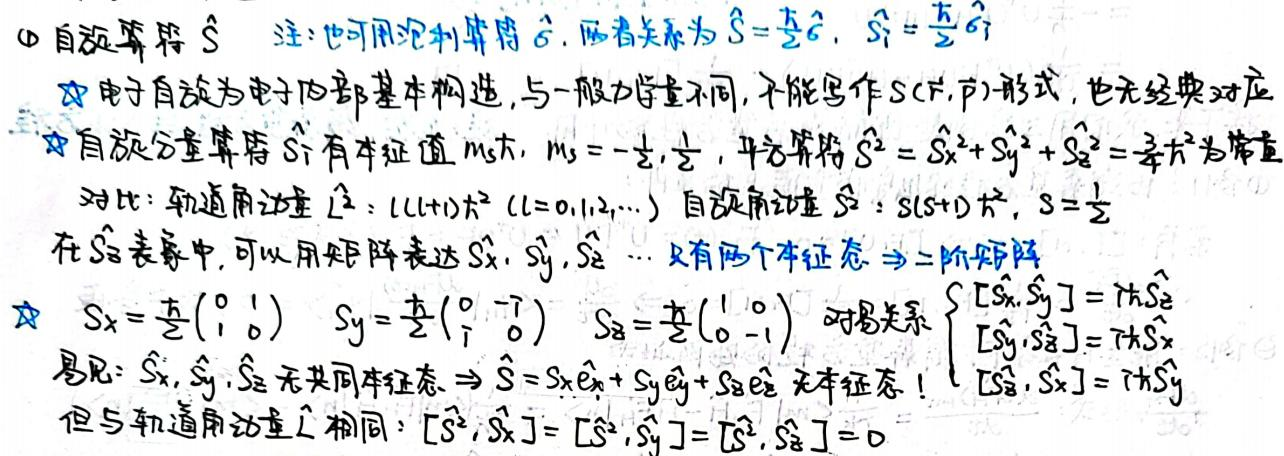
\includegraphics[width=0.32\textwidth]{images/10.png}
    \vspace{-0.6cm}
\end{figure}
\begin{figure}[H]
    \vspace{-0.5cm}
    \centering
    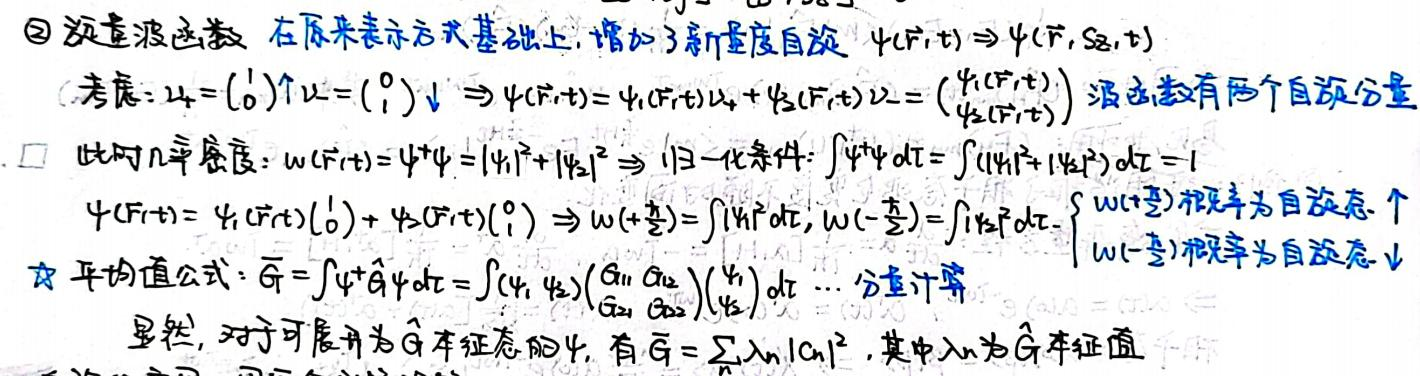
\includegraphics[width=0.32\textwidth]{images/11.png}
    \vspace{-0.6cm}
\end{figure}
\bluetext{角动量的合成}

有时用总角动量(耦合)表象比较方便,即$\hat{J} = \hat{J_1}+\hat{J_2}$\\
共同本征函数系为基底的表象称为耦合表象\\
此时表示$J^2,J_z$的本征函数为$|j,m\rangle$\\
$\hat{J}^2$本征值为$j(j+1)\hbar^2$,$J_z$本征值为$m\hbar$\\
$j=0,1,2,\dots or \frac{1}{2},\frac{3}{2},\dots, m=-j,-j+1,\dots,j$\\
角动量合成法则:\\$j=j_1+j_2,j_1+j_2-1,\dots,|j_1-j_2|$,
\\$m=-j,-j+1,\dots,j$\\
电子的总角动量L+S:\\
\begin{figure}[H]
    \vspace{-0.5cm}
    \centering
    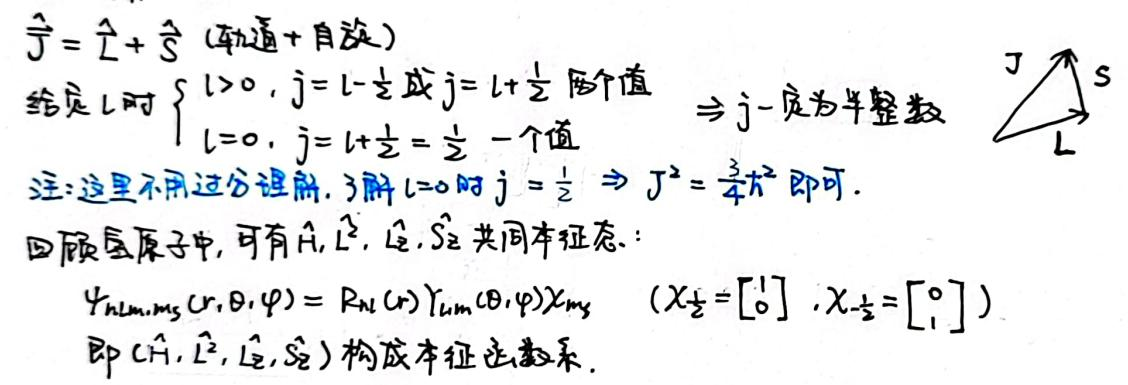
\includegraphics[width=0.32\textwidth]{images/12.png}
    \vspace{-0.6cm}
\end{figure}

\redtext{其他}:\\
$\int_{-\infty}^{+\infty}e^{-ax^2}dx = \sqrt{\frac{\pi}{a}}$\\
$\int_{0}^{+\infty}x^ne^{-ax}dx = \frac{n!}{a^{n+1}}$\\
$\int_{0}^{+\infty}x^{2n}e^{-ax^2}dx = \frac{(2n-1)!!}{2^{n+1}}\sqrt{\frac{\pi}{a^{2n+1}}}$\\
$\int_{0}^{+\infty}x^{2n-1}e^{-ax^2}dx = \frac{(n-1)!}{2a^{n}}$\\
$\int_{-\infty}^{+\infty}cos(wx)e^{-ax^2}dx = \sqrt{\frac{\pi}{a}}e^{-\frac{w^2}{4a}}$\\
散度定理$\int_V \nabla\cdot\vec{A}dV = \oint_S \vec{A}\cdot d\vec{S}$\\
旋度定理$\int_S \nabla\times\vec{A}\cdot d\vec{S} = \oint_C \vec{A}\cdot d\vec{l}$\\
\end{multicols}
\end{document}